\chapter{Цели и задачи работы}
\textbf{Цель работы} --- построение доверительных интервалов для математического ожидания и дисперсии нормальной случайной величины.
\textbf{Содержание работы:}
\begin{enumerate}
\item Для выборки объёма n из генеральной совокупности X реализовать в виде программы на ЭВМ:
\begin{enumerate}
\item вычисление точечных оценок $\hat{\mu}(\overrightarrow{x_{n}})$ и $S^{2}(\overrightarrow{x_{n}})$ математического ожидания MX и дисперсии DX соответственно;
\item вычисление нижней и верхней границ $\underline{\mu}(\overrightarrow{x_{n}})$, $\overline{\mu}(\overrightarrow{x_{n}})$ для\\
$\gamma$-доверительного интервала для математического ожидания MX;
\item вычисление нижней и верхней границ $\underline{\sigma}^{2}(\overrightarrow{x_{n}})$, $\overline{\sigma}^{2}(\overrightarrow{x_{n}})$ для $\gamma$-доверительного интервала для дисперсии DX;
\end{enumerate}
\item вычислить $\hat\mu$, $S^2$ из индивидуального варианта;
\item для заданного пользователем уровня доверия $\gamma$ и N - объёма выборки из индивидуального варианта:
\begin{enumerate}
\item на координатной плоскости Oyn построить прямую $y =\hat\mu(\ora{x}_{N})$, также графики функций $y = \hat\mu(\ora{x_{n}}), y = \uline{\mu}(\ora{x_{n}}), y = \oline{\mu}(\ora{x_{n}})$ как функций объёма n выборки, где n изменяется от 1 до N. 
\item на другой координатной плоскости Ozn построить прямую $z = S^2(\ora{x_{N}})$, также графики функций $z = S^2(\ora{x\lind{n}}))$, $z = \uline{\sigma\pwr{2}}(\ora{x\lind{n}})$ и $z = \oline{\sigma\pwr{2}}(\ora{x}\lind{n})$ как функций объёма n выборки, где n изменяется от 1 до N. 
\end{enumerate}
\end{enumerate}

\chapter{Теоретическая часть}
\section{Формулы для вычисления точечных оценок математического ожидания и дисперсии}
Пусть $(x_{1}, ..., x_{n})$ - некая случайная выборка.

Оценка $\hat{\mu}$ (u\_x) для математического ожидания MX вычисляется как $\hat{\mu}(\overrightarrow{X_{n}}) = \overline{X_{n}} = \frac{1}{n}\sum\limits_{i=1}^{n} X_{i}$.

Оценка $S^{2}$ (S\_2\_x) для дисперсии (несмещённая) вычисляется как $S^{2}(\overrightarrow{X_{n}}) = \frac{1}{n - 1}\sum\limits_{i=1}^{n}(X_{i} - \oline{X_{n}})^{2}$.

\section{Определение $\gamma$-доверительного интервала для значения параметра распределения случайной величины}
Пусть $\ora{X\lind{n}}$ - случайная выборка n из генеральной совокупности X с функцией распределения $F(x;\theta)$, зависящей от параметра $\theta$, значение которого неизвестно.

Тогда интервальной оценкой с коэффициентов доверия $\gamma$ ($\gamma$-доверительной интервальной оценкой) параметра $\theta$ называют пару статистик $\uline{\theta}\ora{X\lind{n}}, \oline{\theta}\ora{X\lind{n}}$ таких, что:\\
$P\{\uline{\theta}\ora{X\lind{n}} < \theta < \oline{\theta}\ora{X\lind{n}}\} = \gamma$\\

Интервал $(\uline\theta(\ora{X_{n}}), \oline\theta(\ora{X_{n}}))$ называют интервальной оценкой для параметра $\theta$ с коэффициентов доверия $\gamma$, а $\uline\theta(\ora{X_{n}}), \oline\theta(\ora{X_{n}})$ называют соответственно нижней и верхней графницами интервальной оценки. Смысл интервальной оценки состоит в том, что она представляет интервал со случайными границами, который с заданной вероятностью $\gamma$ накрывает неизвестное истинное значение параметра $\gamma$.

Интервал $(\uline\theta(\ora{X_{n}}), \oline\theta(\ora{X_{n}}))$ называют доверительным интервалом для параметра с коэффициентов доверия $\gamma$, где $\ora{x\lind{n}}$ - любая реализация случайной выборки $\ora{X\lind{n}}$.

\section{Формулы для вычисления границ $\gamma$-доверительного интервала для математического ожидания и дисперсии}
Для вычисления верхней и нижней границы $\gamma$-доверительного интервала для математического ожидания используются следующие формулы:\\
$\uline{\mu}(\ora{X\lind{n}}) = \oline{X} - \frac{S(\ora{X})}{\sqrt{n}}t\lind{1 - \alpha}(n - 1)$ (u\_low)\\
$\oline{\mu}(\ora{X\lind{n}}) = \oline{X} - \frac{S(\ora{X})}{\sqrt{n}}t\lind{1 - \alpha}(n - 1)$ (u\_high)\\
$\oline{X}$ - точечная оценка математического ожидания\\
$S^{2}(\ora{X})$ - точечная оценка дисперсии\\
n - объём выборки\\
$\gamma$ - уровень доверия\\
$t\lind{1 - \alpha}$ - квантиль уровня $1 - \alpha$ для распределения Стьюдента с n - 1 степенями свободы, $\alpha = \frac{1 - \gamma}{2}$\\

Для вычисления верхний и нижней границы $\gamma$-доверительного интервала для дисперсии:\\
$\uline{\sigma}^{2}(\ora{x_{n}}) = \frac{(n - 1)S^{2}(\ora{X})}{\chi^{2}_{1 - \alpha}(n - 1)}$  (sigma\_2\_low)\\
$\oline{\sigma}^{2}(\ora{x_{n}}) = \frac{(n - 1)S^{2}(\ora{X})}{\chi^{2}_{\alpha}(n - 1)}$ (sigma\_2\_high)\\
$S^{2}(\ora{X})$ - точечная оценка дисперсии\\
n - объём выборки\\
$\gamma$ - уровень доверия\\
$\chi\lind{1 - \alpha}(n - 1)$ - квантиль уровня $1 - \alpha$ для распределения Стьюдента с n - 1 степенями свободы, $\alpha = \frac{1 - \gamma}{2}$\\

\chapter{Практическая часть}

\section{Результаты работы для выборки по варианту}
\begin{lstlisting}
Lab 2
n = 120
u_x = -1.6046
S_2_x = 1.0341
u_low = -1.7585
u_high = -1.4507
sigma_2_low = 0.8460
sigma_2_high = 1.2979
\end{lstlisting}
\newpage

\begin{figure}[H]
	\center{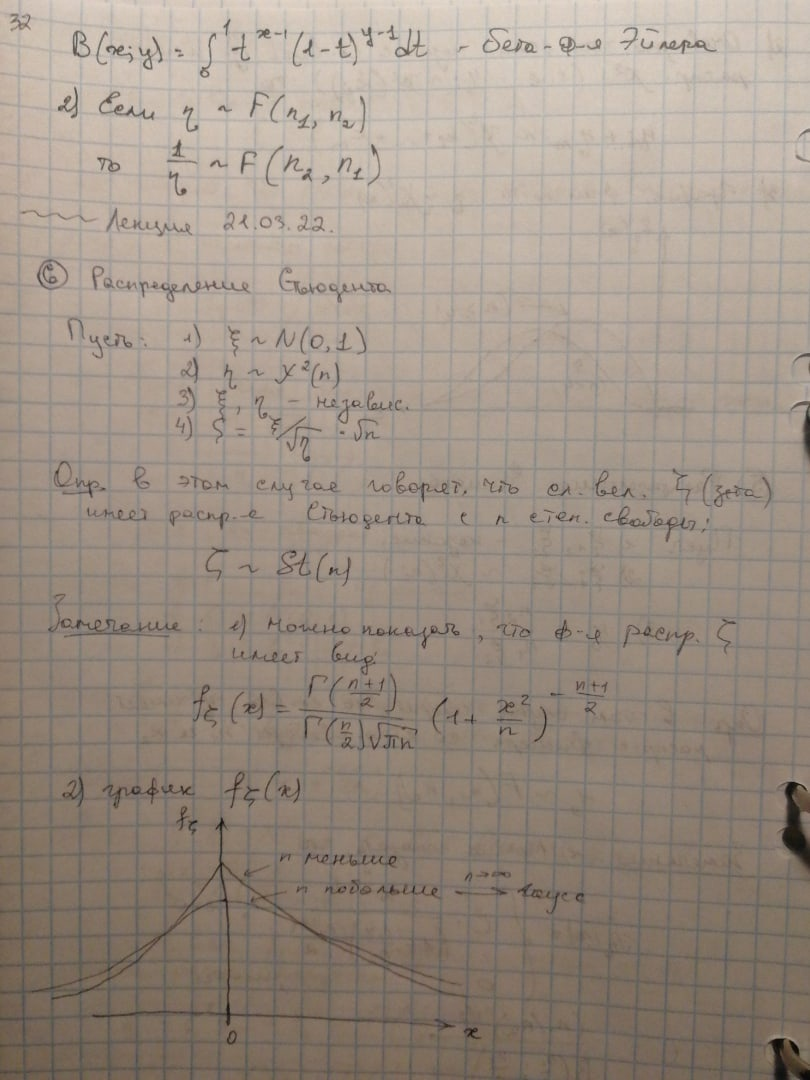
\includegraphics[scale=1.3]{1}}
\end{figure}

\begin{figure}[H]
	\center{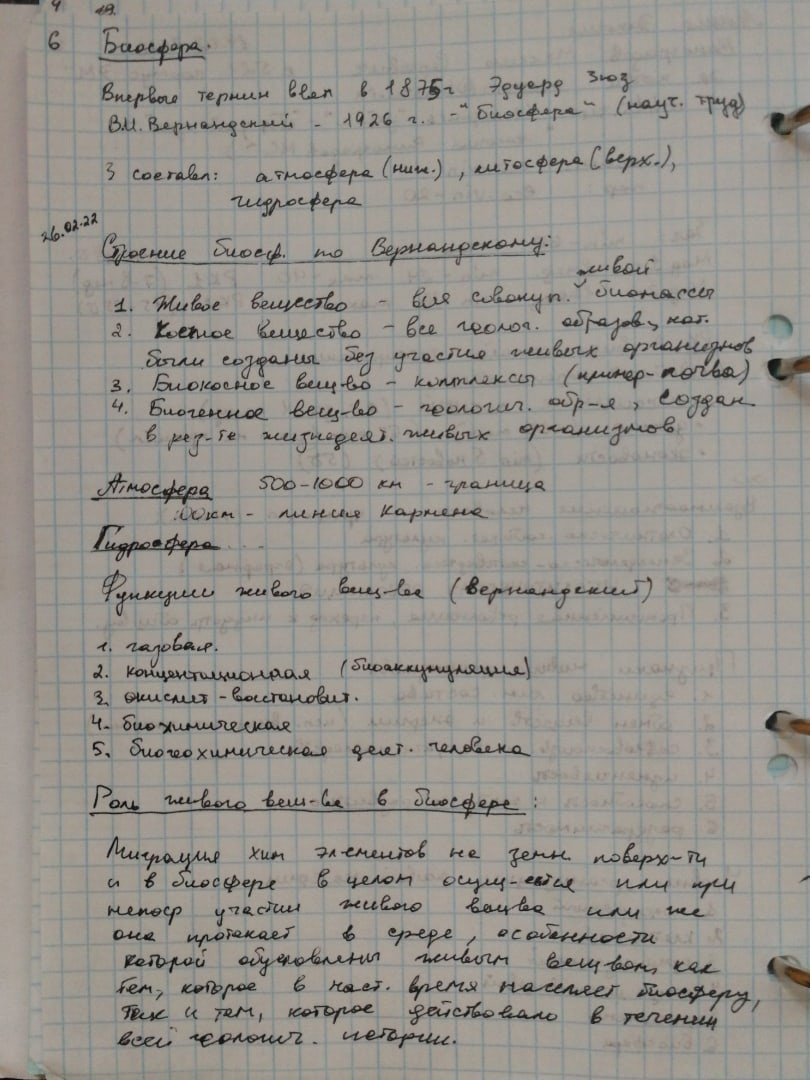
\includegraphics[scale=1.3]{2}}
\end{figure}

\begin{figure}[H]
	\center{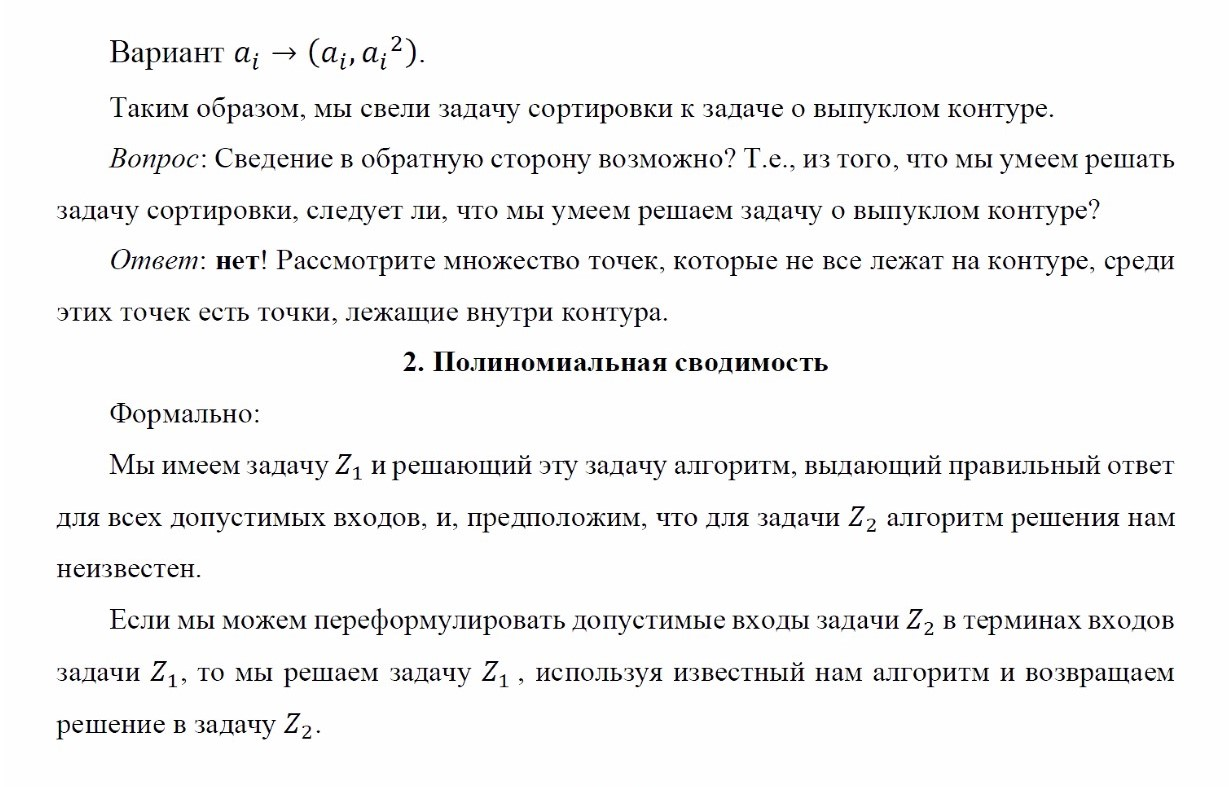
\includegraphics[scale=1.3]{3}}
\end{figure}

\newpage

\section{Листинг программы}
\begin{lstlisting}
disp("Lab 2")
pkg load statistics

# Выборка
x_unsorted = [-0.23,-1.03,-4.11,-0.65,-2.58,-0.79,-1.53,-0.18,-2.79,-1.97,-2.21,-1.59,-0.22,-3.18,-1.18,-1.42,-1.29,-2.22,-0.82,-1.87,-2.30,-0.94,-0.74,-2.45,-1.40,-2.09,-0.68,0.02,-1.80,-2.25,-1.19,-2.17,-1.89,-1.14,-1.50,-1.76,-0.69,-2.21,-1.65,-1.51,-2.11,-2.24,-0.72,0.94,-0.67,-2.44,-2.27,-1.33,-3.03,-0.42,-2.86,-2.00,-1.37,-1.90,-2.80,-0.89,-2.04,-1.66,-0.14,-2.79,-0.21,-1.29,-2.81,-0.29,-1.55,-0.45,-1.16,-3.96,-3.77,-3.36,-1.81,0.13,-2.61,-3.69,-3.00,-2.61,-0.74,-0.41,-0.78,-1.49,-1.89,-1.24,-0.00,-2.72,-1.69,-1.25,-1.59,0.20,-1.08,-2.42,-3.14,-2.54,-2.09,-2.51,-2.65,-2.42,-1.30,-0.65,1.40,-2.33,-1.97,-0.54,-1.13,-2.04,0.77,-1.03,-1.55,-1.47,-0.09,-2.11,-2.08,-1.79,-1.36,-1.92,-3.04,-1.08,-1.67,-2.11,-1.99,-1.64];

# Сортировка массива данных
x = sort(x_unsorted);

# Нахождение длины массива
n = length(x)

# Оценка матожидания
function res = u_x_f(x)
  res = (1/numel(x))*sum(x);
endfunction
u_x = u_x_f(x)

# Несмещённая оценка дисперсии
function res = S_2_x_f(x, u_x)
  val = 0;
  for i = 1:numel(x)
    val +=(x(i) - u_x)*(x(i) - u_x);
  endfor
  res = val*(1/(numel(x) - 1));
endfunction
S_2_x = S_2_x_f(x, u_x)

gamma = 0.95;

# Нижняя граница доверительного интервала для матожидания
# tinv - функция распределения инверсии t студента
function res = u_low_f(u_x, S_2_x, n, gamma)
  alpha = (1 - gamma)/2;
  res = u_x - sqrt(S_2_x) / sqrt(n) * tinv(1 - alpha, n - 1);
endfunction

# Верхняя граница доверительного интервала для матожидания
function res = u_high_f(u_x, S_2_x, n, gamma)
  alpha = (1 - gamma)/2;
  res = u_x + sqrt(S_2_x) / sqrt(n) * tinv(1 - alpha, n - 1);
endfunction

u_low = u_low_f(u_x, S_2_x, n, gamma)
u_high = u_high_f(u_x, S_2_x, n, gamma)

# Нижняя граница доверительного интервала для дисперсии
function res = sigma_2_low_f(S_2_x, gamma, n)
  alpha = (1 - gamma)/2;
  res = ((n - 1) * S_2_x) / chi2inv(1 - alpha, n - 1);
endfunction

# Верхняя граница доверительного интервала для дисперсии
function res = sigma_2_high_f(S_2_x, gamma, n)
  alpha = (1 - gamma)/2;
  res = ((n - 1) * S_2_x)/chi2inv(alpha, n - 1);
endfunction

sigma_2_low = sigma_2_low_f(S_2_x, gamma, n)
sigma_2_high = sigma_2_high_f(S_2_x, gamma, n)

x = x_unsorted;
y = [];
# Построение графиков
figure();
hold on;
x_n = 2:1:n;
for i = 1:numel(x_n)
  y(i) = u_x_f(x);
endfor

plot(x_n, y, 'r');
xlabel('n')
ylabel('y')

x_n = 2:1:n;
for i = 2:numel(x)
  y(i - 1) = u_x_f(x(2:i));
endfor
plot(x_n, y, 'b');
xlabel('n')
ylabel('y')

for i = 2:numel(x)
  u_x = u_x_f(x(2:i));
  S_2_x = S_2_x_f(x(2:i), u_x);
  y(i - 1) = u_low_f(u_x, S_2_x, i, gamma);
endfor

plot(x_n, y, 'g');
xlabel('n')
ylabel('y')

for i = 2:numel(x)
  u_x = u_x_f(x(2:i));
  S_2_x = S_2_x_f(x(2:i), u_x);
  y(i - 1) = u_high_f(u_x, S_2_x, i, gamma);
endfor

plot(x_n, y, 'c');
xlabel('n')
ylabel('y')
legend ({"u\\_x", "u\\_x от n", "u\\_low от n", "u\\_high от n"}, "location", "north");
hold off;

# Графики для дисперсии
figure();
hold on;
x_n = 2:1:n;
for i = 2:numel(x)
  y(i - 1) = S_2_x_f(x, u_x);
endfor
plot(x_n, y, 'r');
xlabel('n')
ylabel('y')

x_n = 2:1:n;
for i = 2:numel(x)
  u_x = u_x_f(x(2:i));
  y(i - 1) = S_2_x_f(x(2:i), u_x);
endfor
plot(x_n, y, 'b');
xlabel('n')
ylabel('y')

for i = 2:numel(x)
  u_x = u_x_f(x(2:i));
  S_2_x = S_2_x_f(x(2:i), u_x);
  y(i - 1) = sigma_2_low_f(S_2_x, gamma, i);
endfor

plot(x_n, y, 'g');
xlabel('n')
ylabel('y')

for i = 2:numel(x)
  u_x = u_x_f(x(2:i));
  S_2_x = S_2_x_f(x(2:i), u_x);
  y(i - 1) = sigma_2_high_f(S_2_x, gamma, i);
endfor

plot(x_n, y, 'c');
xlabel('n')
ylabel('y')
legend ({"S\\_2\\_x", "S\\_2\\_x от n", "sigma\\_2\\_low от n", "sigma\\_2\\_high от n"}, "location", "north");
hold off;

# Графики для дисперсии с n = 10
figure();
hold on;
x_n = 2:1:n;
for i = 2:numel(x)
  y(i - 1) = S_2_x_f(x, u_x);
endfor
plot(x_n(10:numel(x_n)), y(10:numel(y)), 'r');
xlabel('n')
ylabel('y')

x_n = 2:1:n;
for i = 2:numel(x)
  u_x = u_x_f(x(2:i));
  y(i - 1) = S_2_x_f(x(2:i), u_x);
endfor
plot(x_n(10:numel(x_n)), y(10:numel(y)), 'b');
xlabel('n')
ylabel('y')

for i = 2:numel(x)
  u_x = u_x_f(x(2:i));
  S_2_x = S_2_x_f(x(2:i), u_x);
  y(i - 1) = sigma_2_low_f(S_2_x, gamma, i);
endfor

plot(x_n(10:numel(x_n)), y(10:numel(y)), 'g');
xlabel('n')
ylabel('y')

for i = 2:numel(x)
  u_x = u_x_f(x(2:i));
  S_2_x = S_2_x_f(x(2:i), u_x);
  y(i - 1) = sigma_2_high_f(S_2_x, gamma, i);
endfor

plot(x_n(10:numel(x_n)), y(10:numel(y)), 'c');
xlabel('n')
ylabel('y')
legend ({"S\\_2\\_x", "S\\_2\\_x от n", "sigma\\_2\\_low от n", "sigma\\_2\\_high от n"}, "location", "north");
hold off;
\end{lstlisting}